% This is samplepaper.tex, a sample chapter demonstrating the
% LLNCS macro package for Springer Computer Science proceedings;
% Version 2.20 of 2017/10/04
%
\documentclass[runningheads]{llncs}
%
\usepackage{graphicx}
% Used for displaying a sample figure. If possible, figure files should
% be included in EPS format.
%
% If you use the hyperref package, please uncomment the following line
% to display URLs in blue roman font according to Springer's eBook style:
% \renewcommand\UrlFont{\color{blue}\rmfamily}

\usepackage{fancyhdr} % Used for page numbers
\usepackage{float} % Lets you prevent LaTeX from repositioning images and tables using [H] specifier.

% Algorithms
\usepackage{algpseudocode}
\usepackage{algorithm}
\usepackage{amsmath}

% Tab
\usepackage{multirow}

\pagestyle{plain}
\fancyhf{} % Clear header and footer
\cfoot{\thepage} % Page number in the right footer

\begin{document}


%
\title{Efficient and secure implementation of AES-GCM in Jasmin}


%
%\titlerunning{Abbreviated paper title}
% If the paper title is too long for the running head, you can set
% an abbreviated paper title here
%
\author{Noah Candaele\inst{1} \and Anthony Iozzia\inst{1} \and Sid Touati\inst{2} (supervisor) \and Benjamin Grégoire\inst{2} (co-supervisor) \and Jean-Christophe Léchenet\inst{2} (co-supervisor)}


%
\authorrunning{F. Author et al.}
% First names are abbreviated in the running head.
% If there are more than two authors, 'et al.' is used.
%
\institute{
Master 2 Cybersecurity, Université Côte d'Azur, Sophia-Antipolis, France\\
\email{\{noah.candaele,anthony.iozzia\}@etu.univ-cotedazur.fr}
\and 
Inria research institute, Sophia-Antipolis, France\\
\email{\{sid.touati,benjamin.gregoire,jean-christophe.lechenet\}@inria.fr}
}



%
\maketitle              % typeset the header of the contribution
%

\begin{center}
    Development project conducted from October 2023 to February 2024.
\end{center}

\thispagestyle{plain} % display page nb also on first page


\begin{abstract}
This report presents the implementation of the Advanced Encryption Standard with Galois/Counter Mode (AES-GCM) in Jasmin, marking a significant stride towards the development of efficient and secure cryptographic code. Jasmin, a dedicated cryptographic programming language, provides a unique blend of high-level and low-level features, offering a flexible and secure environment for cryptographic operations.

The implementation encompasses AES in Jasmin, leveraging AES-NI for hardware acceleration. The focus then shifts to AES-GCM, implemented in Jasmin using regular primitives. This work not only strengthens the cryptographic functionality in Jasmin but also establishes a foundational step towards the creation of high-assurance, efficient, and secure code.

 In addressing potential threats, the report emphasizes the significance of constant-time execution to mitigate vulnerabilities, contributing to the overall security of cryptographic systems. The successful implementation of AES-GCM in Jasmin represents a promising start in the pursuit of efficient and secure cryptographic solutions, fostering the advancement of digital communication security.

\keywords{Jasmin \and Cryptography \and AES-GCM \and High-assurance.}
\end{abstract}

%

\newpage
\section{Introduction}

Cryptography, a specialized branch of mathematics and computer science, has distinct needs that differentiate it from general-purpose programming. Cryptographic programs require careful attention, such as focusing on certifying the code and ensuring stable performance to prevent security breaches. It's crucial to prioritize the strength and reliability of cryptographic implementations to protect sensitive information and prevent potential attacks.

Recognizing the distinctive nature of cryptographic applications, there has been a concerted effort in the development of programming languages specifically tailored to address the intricate demands of cryptography. These specialized languages aim to provide a secure and efficient environment for cryptographic operations, acknowledging the critical role they play in securing digital communication, financial transactions, and sensitive data.

This scientific report explores various cryptographic programming languages, examining their unique features, design principles, and performance traits. It investigates advanced algorithms, particularly focusing on the widely adopted Advanced Encryption Standard (AES) and the authenticated encryption algorithm AES-GCM (Galois/Counter Mode), both integral components of cryptographic systems.

Following this exploration, the report highlights the distinctiveness of Jasmin, a dedicated cryptographic language, and emphasizes the significance of its role in advancing cryptographic functionality. The main goal of the project becomes clear: to implement the AES-GCM algorithm within Jasmin. This implementation aims to enhance cryptographic operations and underscore the potential for further advancements in securing digital communication, financial transactions, and sensitive data. Finally, the report will delve into the details of implementing the AES-GCM algorithm within the Jasmin language.


\section{Languages dedicated to cryptography}

\subsection{Some languages}
\subsubsection{HACL*:}
HACL*~\cite{hacl_star_paper} (High-Assurance Cryptographic Library) is a programming language designed for writing high-assurance cryptographic code. It focuses on providing a formally verified and secure environment for cryptographic implementations, aiming to eliminate vulnerabilities and exploits in sensitive applications. One of its primary advantages is its emphasis on formal verification techniques, which enable mathematical proofs of code correctness, enhancing the overall security of cryptographic systems. HACL* supports a wide range of cryptographic primitives and is implemented in F*, a functional programming language that allows expressive specifications and formal reasoning. However, its disadvantages include a potentially steep learning curve due to the need for developers to understand formal methods and the limited scope of applications, as HACL* is specifically tailored for cryptographic tasks, making it less suitable for general-purpose programming. Additionally, the verification process can be resource-intensive, impacting development time.


\subsubsection{Qhasm:}
%Quantum High-Assurance Software Methodology
 Qhasm~\cite{qhasm} is a project that aims to develop tools and interfaces for the high-speed generation of professional-quality software for various applications, particularly in the field of quantum computing.
However, it is important to note that Qhasm is in prototype form since 2007, and there are significant reasons for not using it in professional settings:
\begin{itemize}
    \item Tool Deficiencies: The existing Qhasm tools and interfaces, while capable of producing high-speed software, are not themselves of professional quality. They have many known deficiencies and areas that need improvement.
    \item Planned Rewrites: Each of the Qhasm tools has at least one complete rewrite planned, indicating ongoing development and potential instability in the current versions.
    \item Instability of .q language: The .q language used in Qhasm is not stable. If developers write code in .q files, they should anticipate extensive modifications for future Qhasm releases.
\end{itemize}


\subsubsection{Cryptol:} 
Cryptol~\cite{cryptol} is a domain-specific language specifically designed for specifying and verifying cryptographic algorithms. It provides a concise and expressive syntax for describing cryptographic operations and protocols, allowing for formal verification and analysis of their security properties. 

One notable advantage of Cryptol is its ability to bridge the gap between high-level algorithmic descriptions and their low-level implementations, facilitating a more systematic and secure development process. Cryptol's type system aids in catching potential vulnerabilities early in the design phase, contributing to enhanced security. Additionally, Cryptol supports automated testing and formal verification, enabling developers to ensure the correctness and robustness of cryptographic code. 

However, challenges exist, such as a potential learning curve due to the specialized nature of the language. Integrating Cryptol into existing development workflows may require effort, and the ecosystem around Cryptol tools may not be as extensive as more widely adopted programming languages. Nonetheless, Cryptol stands out as a valuable tool for building and verifying secure cryptographic systems.

\subsection{Why we choose the Jasmin programming language}
Jasmin~\cite{jasmin_paper}, as a verified programming language and compiler, stands out in the field of high performance and high-assurance cryptography. This platform offers a flexible programming environment that combines both high-level and low-level features. Programmers using Jasmin have the ability to optimize crucial aspects for performance, such as instruction selection and register allocation, while exploiting high-level concepts such as variables, functions, tables and loops to organize and check their code.

Jasmin benefits from a formal semantics that facilitates rigorous reasoning on the behavior of programs. This semantics is defined in Coq and can be used to directly interpret Jasmin programs.

The Jasmin compiler generates an efficient and predictable assembly code that preserves the properties of the source program.

The Jasmin workbench uses the EasyCrypt tool set for formal verification. Jasmin programs can be translated into corresponding EasyCrypt programs to prove functional correction, cryptographic security or security against auxiliary channel attacks (constant time).

Jasmin combines the best of all worlds: high-level language with high performance and high assurance. For these reasons, we will use Jasmin as the programming language for our implementations of cryptographic algorithms.



\section{Cryptography's Role in Digital Security}

The rapid evolution of Information and Communication Technology (ICT) has elevated the internet to a central platform for information in the 21st century. Despite this, ensuring the confidentiality, integrity, and availability of information transmitted over public networks remains a persistent challenge. Various methods, including information hiding through watermarking and steganography, as well as cryptographic techniques, have been extensively studied to enhance the security of data exchanged over unsecured networks.

Within the realm of cryptography, the primary objective is to safeguard information by rendering a secret message indecipherable to unauthorized parties, allowing only the sender and intended recipient to access its contents. This is achieved through the utilization of one or more secret keys. Cryptographic techniques can be broadly categorized as symmetric, where the same key is used for both encryption and decryption, or asymmetric, where distinct keys perform these functions.

Symmetric cryptographic techniques are particularly advantageous when securing substantial volumes of data. Indeed, asymmetric algorithms are more computationally intensive. Noteworthy examples of symmetric cryptographic algorithms include the Data Encryption Standard (DES), Triple DES, and the widely adopted Advanced Encryption Standard (AES). Among these, AES has emerged as the most prevalent and extensively utilized method for ensuring the security of sensitive information in the digital landscape.

\subsection{The Advanced Encryption Standard (AES)}

The Advanced Encryption Standard algorithm, established as the encryption standard for digital data by the US National Institute of Standards and Technology (NIST), is a symmetric key algorithm. Operating as an iterative round block cipher, it processes 128-bit plaintext using key lengths of 128, 192, and 256 bits. The chosen key length dictates the number of encryption and decryption rounds, 10, 12, and 14 rounds. It is generally understood that a larger key length enhances cryptographic strength. The AES algorithm, developed by a team led by Vincent Rijmen and Joan Daemen, consists of four invertible transformations: SubBytes, ShiftRows, MixColumns, and AddRoundKey.

Each of these transformations is applied in every encryption round, except for the last round, where the MixColumns transformation is deliberately excluded. This omission in the final round aims to maintain symmetry between the encryption and decryption processes. The transformations can be described as follows:

\begin{itemize}
    \item SubBytes Transformation: During this phase, each byte in the block is substituted with a corresponding byte from a fixed substitution table (S-box). This non-linear substitution, facilitated by the S-box, introduces intricacy to the algorithm, fortifying its resistance against cryptanalysis.
    \item ShiftRows Transformation: This operation entails shifting the rows of the block, contributing to diffusion and introducing complexity. The offset for each row's shift varies, enhancing the overall confusion in the encrypted data.
    \item MixColumns Transformation: In this step, a mathematical operation is applied to each column of the block. This operation fosters diffusion across columns, significantly contributing to the algorithm's resistance against linear attacks.
    \item AddRoundKey Transformation: The final step involves a bitwise XOR operation between a round key, generated from the original encryption key using a key schedule, and the state matrix. This step introduces the key into the encryption process, ensuring that each round employs a unique portion of the key, thereby boosting the overall security of the algorithm.
\end{itemize}

Collectively, these transformations establish a robust and secure encryption process. The deliberate symmetry in the final round ensures consistency between encryption and decryption procedures.

\subsection{Algorithm specification}



The input block, output block, and State of AES are all 128 bits. We define $N_b = 4$, which is the number of 32-bit words, or columns, in the State structure.

The Cipher Key ($K$) can have the lengths 128, 192, and 256 bits. These lengths are denoted by $N_k = 4, 6,$ or $8$, indicating the number of 32-bit words, or columns, that compose the Cipher Key.

The AES algorithm adapts to different key sizes, influencing the number of rounds ($N_r$) in its cryptographic process, which are defined as $N_r = 10$ for $N_k = 4$, $N_r = 12$ for $N_k = 6$, and $N_r = 14$ for $N_k = 8$.

The Key-Block-Round combinations are given in Fig. \ref{fig:table_key_block_round_combinations}. The AES encryption algorithm can be found in Algorithm \ref{fig:algo_aes_encrypt}. The AES decryption algorithm can be found in Algorithm \ref{fig:algo_aes_decrypt}.


\begin{figure}[ht]
    \centering
    \begin{tabular}{c|c|c|c|}
        \cline{2-4}
        & \textbf{\begin{tabular}[c]{@{}c@{}}Key Length\\ (Nk words)\end{tabular}} & \textbf{\begin{tabular}[c]{@{}c@{}}Block Size\\ (Nb words)\end{tabular}} & \textbf{\begin{tabular}[c]{@{}c@{}}Number of\\ Rounds\\ (Nr)\end{tabular}} \\ \hline
        \multicolumn{1}{|c|}{\textbf{AES-128}} & 4 & 4 & 10 \\ \hline
        \multicolumn{1}{|c|}{\textbf{AES-192}} & 6 & 4 & 12 \\ \hline
        \multicolumn{1}{|c|}{\textbf{AES-256}} & 8 & 4 & 14 \\ \hline
    \end{tabular}
    \caption{Key-Block-Round Combinations}
    \label{fig:table_key_block_round_combinations}
\end{figure}


\begin{algorithm}[hbt!]
\caption{Pseudocode for AES encryption. Src: NIST FIPS~\cite{AES_NIST}}
\begin{algorithmic}[1] % [1] = line numbers
    \Procedure{AesEncrypt}{$\text{in}, \text{Nr}, \text{w}$}
        \State $\text{state} \gets \text{in}$
        \State $\text{state} \gets \Call{AddRoundKey}{\text{state}, \text{w}[0..3]}$
        \For{$\text{round}$ \textbf{from} $1$ \textbf{to} $\text{Nr} - 1$}
            \State $\text{state} \gets \Call{SubBytes}{\text{state}}$
            \State $\text{state} \gets \Call{ShiftRows}{\text{state}}$
            \State $\text{state} \gets \Call{MixColumns}{\text{state}}$
            \State $\text{state} \gets \Call{AddRoundKey}{\text{state}, \text{w}[4 \times \text{round}..4 \times \text{round} + 3]}$
        \EndFor
        \State $\text{state} \gets \Call{SubBytes}{\text{state}}$
        \State $\text{state} \gets \Call{ShiftRows}{\text{state}}$
        \State $\text{state} \gets \Call{AddRoundKey}{\text{state}, \text{w}[4 \times \text{Nr}..4 \times \text{Nr} + 3]}$
        \State \Return $\text{state}$
    \EndProcedure
\end{algorithmic}
\label{fig:algo_aes_encrypt}
\end{algorithm}

While AES encryption transforms plaintext into ciphertext through a series of substitution, permutation, and key addition steps, AES decryption reverses this process to recover the original plaintext.

\begin{algorithm}[hbt!]
\caption{Pseudocode for AES decryption. Src: NIST FIPS\cite{AES_NIST}}
\begin{algorithmic}[1] % [1] = line numbers
    \Procedure{AesDecrypt}{$\text{in}, \text{Nr}, \text{w}$}
        \State $\text{state} \gets \text{in}$
        \State $\text{state} \gets \Call{AddRoundKey}{\text{state}, \text{w}[4 \times \text{Nr}..4 \times \text{Nr} + 3]}$
        \For{$\text{round \textbf{from} Nr} - 1$ \textbf{downto} $1$}
            \State $\text{state} \gets \Call{InvShiftRows}{\text{state}}$
            \State $\text{state} \gets \Call{InvSubBytes}{\text{state}}$
            \State $\text{state} \gets \Call{AddRoundKey}{\text{state}, \text{w}[4 \times \text{round}..4 \times \text{round} + 3]}$
            \State $\text{state} \gets \Call{InvMixColumns}{\text{state}}$
        \EndFor
        \State $\text{state} \gets \Call{InvShiftRows}{\text{state}}$
        \State $\text{state} \gets \Call{InvSubBytes}{\text{state}}$
        \State $\text{state} \gets \Call{AddRoundKey}{\text{state}, \text{w}[0..3]}$
        \State \Return $\text{state}$
    \EndProcedure
\end{algorithmic}
\label{fig:algo_aes_decrypt}
\end{algorithm}


\newpage
\subsection{AES Galois Counter Mode (AES-GCM)}

AES-CBC (Cipher Block Chaining) is a mode of operation for the Advanced Encryption Standard (AES). In AES-CBC, each plaintext block is XORed with the previous ciphertext block before encryption. This chaining mechanism introduces dependencies between blocks, enhancing security by preventing identical plaintext blocks from producing identical ciphertext blocks.

\begin{figure}[ht] % ht = auto, H = fixed
    \centering
    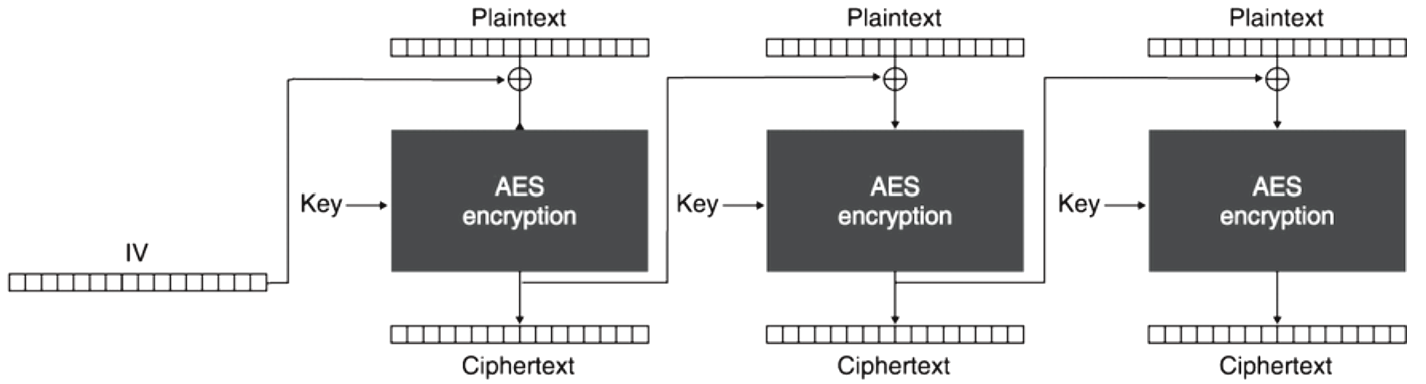
\includegraphics[scale=0.55]{resources/AES_CBC.png}
    \caption{The CBC mode of operation with AES. Src: Real-World Cryptography~\cite{book_real_world_crypto}}
\end{figure}

AES-GCM (Galois/Counter Mode) is another mode of operation for AES. Unlike AES-CBC, GCM combines encryption and authentication, providing both confidentiality and integrity. GCM operates by dividing the data into blocks, encrypting each block using AES in counter mode, and then incorporating an authentication tag. The tag is generated using Galois field multiplication, ensuring data integrity. AES-GCM is widely used in secure communications, such as in TLS (Transport Layer Security) for securing internet connections. It offers efficient and robust protection against both eavesdropping and tampering.

\begin{figure}[ht] % ht = auto, H = fixed
    \centering
    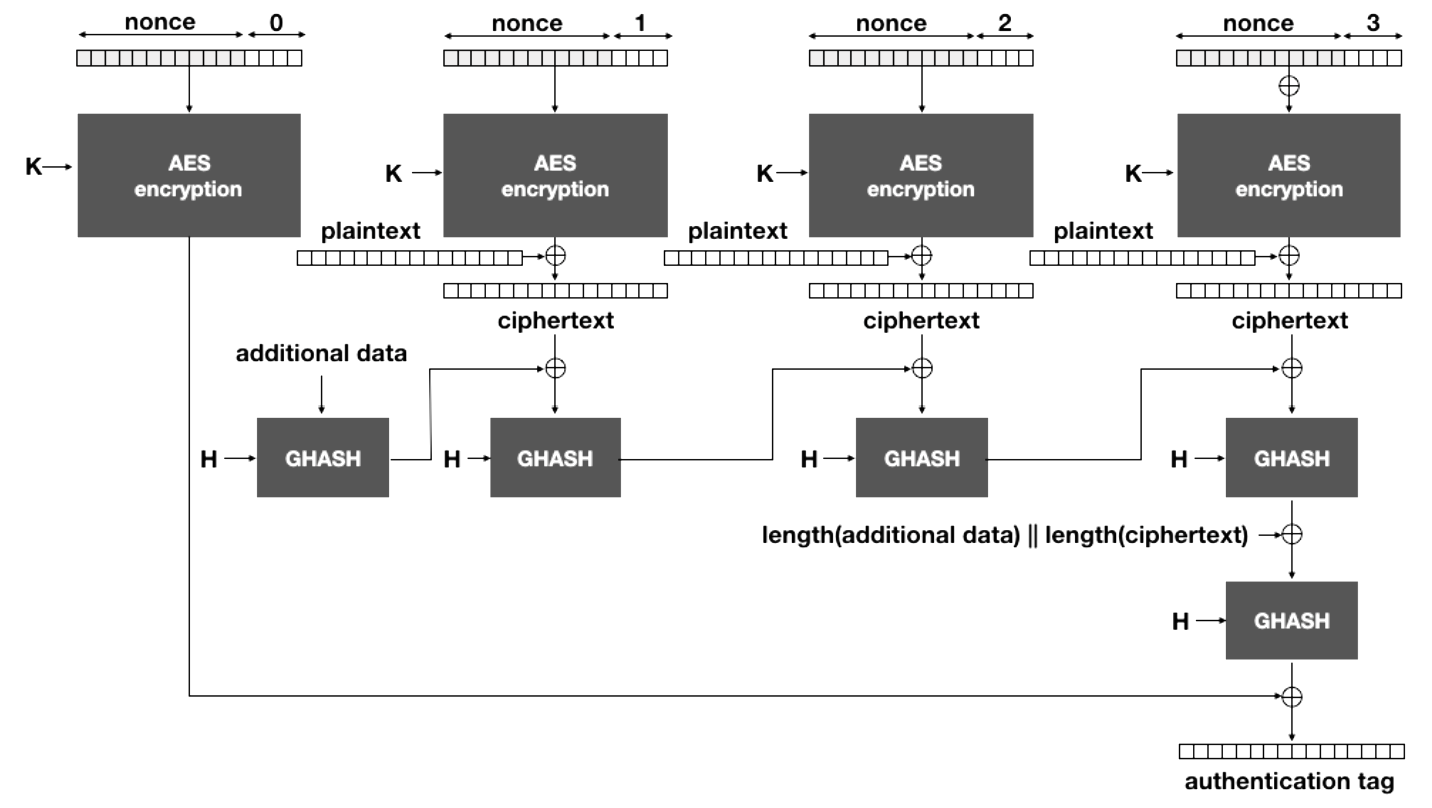
\includegraphics[scale=0.55]{resources/AES_GCM.png}
    \caption{The AES-GCM encryption process. Src: Src: Real-World Cryptography~\cite{book_real_world_crypto}}
\end{figure}

\section{Attacks on high-assurance cryptographic code}

Vulnerabilities can lead to severe consequences, especially for cryptographic code, where the stakes are exceptionally high. High-assurance code undergoes rigorous formal verification processes and adheres to strict development standards, significantly reducing the likelihood of common vulnerabilities. However, potential threats persist, as we will discuss in this section.


\subsection{Side-Channel Attacks}
Side-channel attacks~\cite{paper_side_channel_attacks} exploit information leaked during the execution of cryptographic algorithms.

\subsubsection{Timing attacks}
Timing attacks are a type of side-channel attack that exploits variations in the time taken for specific operations. By carefully measuring the time it takes for a system to perform certain computations, an attacker can gain insights into sensitive information, such as cryptographic keys. The variations in execution time may reveal patterns that allow the attacker to infer details about the underlying data or algorithms.

For example, consider an application that performs user authentication by comparing a hashed user-entered password with the stored hashed password. If the system takes less time to respond when the first character of the password is correct, an attacker could iteratively guess each character and measure the response time. The correct character will result in a slightly longer response time due to the additional computation, allowing the attacker to deduce the correct password one character at a time.

To mitigate timing attacks, algorithms must have constant execution time regardless of input.

\subsubsection{Cache attacks}
Cache attacks are a class of side-channel attacks that exploit variations in cache access times to extract sensitive information. By observing the time it takes to access specific memory locations, an attacker can infer patterns of memory usage, potentially revealing details about confidential data like cryptographic keys. Cache attacks often target the shared cache in multi-core processors, where one core's activities can impact the cache behavior seen by another core.

For example, in a Prime+Probe Attack, an attacker ``primes'' the cache by loading data into it, then measures the time it takes to ``probe'' the cache by accessing certain memory locations. If the target system is performing cryptographic operations, the attacker can correlate the timing information with specific operations, allowing them to deduce sensitive information like cryptographic keys.

Mitigating cache attacks involves using cache-timing-resistant algorithms and implementing secure coding practices. We should aim to minimize observable variations in cache behavior during cryptographic operations. Techniques such as data obfuscation, padding, or algorithmic modifications can be employed to make the access patterns less predictable. Additionally, ensuring that sensitive data is not shared in the same cache line with non-sensitive data can help reduce the risk of cache-based side-channel attacks.

\subsubsection{Power Analysis Attacks}

Power analysis attacks are another subset of side-channel attacks that exploit variations in power consumption during the execution of cryptographic algorithms. By analyzing the power consumption patterns of a device, an attacker can infer information about the internal computations, potentially revealing cryptographic keys or other sensitive data.

There are two primary types of power analysis attacks:

\begin{enumerate}
    \item \textbf{Simple Power Analysis (SPA):} SPA involves analyzing the power consumption of a device over time to identify patterns associated with specific operations. For instance, cryptographic algorithms often involve modular exponentiation, and the power consumption during this operation may exhibit recognizable patterns. Once identified, these patterns can be correlated to extract information about the cryptographic key.
    \item \textbf{Differential Power Analysis (DPA):} DPA is a more sophisticated attack that involves statistical analysis of power consumption differences between different inputs or operations. By observing the power variations, an attacker can notice patterns related to the data being processed. This allows them to deduce information about secret keys or plaintext data.

\end{enumerate}

To counter power analysis attacks, cryptographic implementations can include techniques like constant-time algorithms, which ensure that the power consumption remains constant regardless of the processed data.

However, these types of attacks are out of scope for this project.


\subsection{Mitigating High-Assurance Cryptographic Code Vulnerabilities}
Understanding and mitigating these side-channel vulnerabilities is crucial for developing secure cryptographic code. The most important mitigation that we can implement is ensuring that our algorithms have constant execution time, regardless of input.

\section{Existing cryptographic libraries}

AES-GCM (Advanced Encryption Standard Galois/Counter Mode) represents a sophisticated mode of symmetric encryption, characterized by the use of a single key for encryption and decryption operations. This method merges the AES algorithm with a block counter technique, ensuring both data confidentiality and authentication, which enhances the integrity and security of exchanges. Thanks to its ability to maintain a high level of security while minimizing the footprint of the resources used, AES-GCM emerges as a preferred choice for large-scale encryption, with various implementations covering key lengths of 128, 192 and 256 bits. Among the main libraries offering these implementations are Libsodium and OpenSSL, which enjoy notable recognition in the field of cryptography. The adoption of the Jasmin programming language in our project stems from the lack of implementation of AES-GCM in the Libjade library, written in Jasmin and subject to formal verification, thus highlighting the relevance of our project.

\subsection{Libsodium}

Libsodium is an open-source software library that offers features of modern cryptography. Designed to be easy to use, secure, and powerful, it offers a range of cryptographic primitives, including symmetric encryption, digital signatures, secure hash functions, key exchanges, and more.

This library gained popularity due to its ease of use, robustness and resistance to common cryptographic attacks. Libsodium is implemented in many programming languages, making it accessible to a wide community of developers.

It is often used in applications that require security features such as data privacy, authentication, and integrity of exchanged messages. It is also known for its ease of integration into various projects, making it a popular choice for many applications that require a high level of security.

\subsection{OpenSSL}

OpenSSL is an open-source library widely used in the field of computer security. It provides implementations of a wide range of security protocols, including SSL (Secure Sockets Layer) and TLS (Transport Layer Security), as well as cryptographic functions such as symmetric and asymmetric encryption, secure hashing functions, digital signatures and random number generators.

Thanks to its versatility and robustness, OpenSSL is widely integrated into many software and operating systems to secure network communications, protect sensitive data and ensure the integrity of online transactions. Many web servers, including popular solutions like Apache and Nginx, use OpenSSL to secure HTTPS connections.

Due to its reputation and long history of development, OpenSSL has become an essential part of the Internet security infrastructure. Despite some controversies and vulnerabilities discovered over the years, OpenSSL remains a major reference in the field of online communications security and continues to be widely used and maintained by an active community of developers.

\subsection{Libjade}

Libjade is a cryptographically verified library developed in the Jasmin programming language, accompanied by computer-verified proofs in EasyCrypt. Its main objective is to provide highly reliable implementations of post-quantum cryptographic (PQC) primitives, facilitating the transition to the forthcoming era of asymmetric cryptography. Furthermore, the library includes implementations of diverse symmetric primitives and popular elliptic-curve-based schemes to facilitate the hybrid deployment of PQC.

\section{Programming approach and environment}

The project was implemented using a peer programming approach, where two programmers work together on the same portion of code. This method was chosen to ensure an active revision of the product code, thus promoting a better assimilation of concepts and practices related to the Jasmin language.

In order to ensure the use of the latest versions of the Jasmin compiler and to maintain a stable working environment, we have chosen to adopt the Docker platform. This decision has brought us many benefits, including improved development efficiency and ease of deployment on new machines. Containerization via Docker guarantees the portability of our project, making it independent of the specific configuration of the machine on which it is deployed.

It is relatively simple to install Jasmin on Linux machines. However, its implementation on Windows systems can be quite complex. By using Docker, we establish a bridge between a Linux container and our operating system, thus resolving any compatibility issues. Thus, any new user of our project will not need to perform any configuration other than the installation of our Docker image provided in our Github repository [https://github.com/noahCandaele/jasmin-aes-gcm]. All the steps to install and run the project are available on the same Github, accompanied by concrete examples of use.

\subsection{Docker}

\begin{figure}[ht] % ht = auto, H = fixed
    \centering
    
\includegraphics[scale=0.50]{resources/docker.png}
    \caption{Usage of Docker in our project}
\end{figure}

Docker is an open-source platform for developing, deploying and running applications in software containers. A container is a lightweight, standalone execution unit that encapsulates everything an application needs to work, including code, libraries, dependencies, and environment variables. 

Unlike traditional virtualization, where each application runs on a separate virtual machine with its own operating system, Docker allows multiple containers to run on a single host machine, thus sharing the same OS kernel. This makes Docker containers extremely resource efficient, while ensuring an isolated environment for each application.

Key benefits of Docker include application portability, ease of deployment, and efficient infrastructure management. With Docker, developers can create consistent development environments, test them locally, and deploy them reliably across any infrastructure, whether it’s a laptop, cloud server, or data center.

In summary, Docker simplifies the process of developing and deploying applications using lightweight containers


\section{Structure of the implemented program}

To make our project more accessible to new users, we decided to organize all our different modules in separate folders, acting as a library. For example, the AES module, which allows encryption of a 128-bit block, is placed in the src/aes/ directory and is accompanied by a Makefile to automate compilation and testing. In addition, a README file is available at the root of our project, detailing its context and how to use the project.

\subsection{Structure of a Jasmin program}
We have organized our project with four main types of files:
\begin{itemize}
    \item \texttt{.jinc}: the main Jasmin code that should only be used by Jasmin functions.
    \item \texttt{.jazz}: Jasmin export functions that can be used by other programming languages like \texttt{C}. These functions are the API (Application Programming Interface) of the program.
    \item \texttt{.c}: C programs are used to interact with the Jasmin API of our program: i.e. provide inputs and retrieve outputs.
    \item \texttt{Makefile}: these files describe how the different files should be compiled.
\end{itemize}

\subsection{Our program's modules}

We describe here the different modules of our program. For each module, we have implemented unit tests, to be able to quickly test if all the functions still produce the expected functionality when we update them.

\subsubsection{Utils}
The first part of our project was to create C utility functions, that will help us transform human-readable data to a format that Jasmin can interprete, and vice versa. To exchange data with Jasmin in C, we chose uint8\_t arrays, which are byte arrays. We are working with a x86\_64 architecture, and the x86 processors use little-endian byte ordering. This means that the least significant byte is stored in the lowest storage address, in opposition to big-endian byte ordering, where the most significant byte is stored in the lowest storage address.

Here are the different functions of this module:
\begin{itemize}
    \item \texttt{print\_uint8\_array\_as\_binary}: prints the array contents as binary. It uses the little-endian convention, where least significant bytes are stored at the start of the array, but the bytes are printed in reverse order to present the output in human-readable format.
    \item \texttt{print\_uint8\_array\_as\_hex}: prints the array contents as hexadecimal. Like the previous function, it uses the little-endian convention.
    \item \texttt{print\_uint8\_array\_as\_ascii}: prints the array contents as ASCII characters. Like the previous functions, it uses the little-endian convention.
    \item \texttt{print\_uint8\_array\_as\_\{hex,ascii\}\_in\_order}: print the array contents as hexadecimal and ASCII characters respectively. However, these two functions use the big-endian convention, where most significant bytes are stored at the start of the array, so the bytes are printed in the order of the array to present the output in human-readable format.
    \item \texttt{nb\_bytes\_hex\_string}: takes a string of hexadecimal characters and computes the number of bytes required to store this string in a byte array, i.e. the size of the byte array.
    \item \texttt{compare\_uint8\_arrays}: takes two arrays and their size and compares their contents. The boolean \texttt{true} is returned if the arrays are equal, and \texttt{false} otherwise.
    \item \texttt{convert\_hex\_string\_to\_uint8\_array}: takes a string of hexadecimal characters and converts it to a byte array, using the little-endian convention. The variation with the \texttt{\_in\_order} suffix uses the big-endian convention.
    \item \texttt{convert\_ascii\_string\_to\_uint8\_array}: takes a string of ASCII characters and converts it to a byte array, using the little-endian convention. The variation with the \texttt{\_in\_order} suffix uses the big-endian convention.
    \item \texttt{convert\_uint8\_array\_to\_ascii\_string}: takes a byte array and converts it to a string of ASCII characters, using the little-endian convention. The variation with the \texttt{\_in\_order} suffix uses the big-endian convention.
\end{itemize}

\subsubsection{AES}
The AES section of this project has been slightly modified from the version proposed by Vincent Laporte during the cybersecurity summer school ``Cyber in Nancy'' in 2022~\cite{cyber_in_nancy}. This version of AES uses sets of instructions specific to this cryptographic algorithm, known as AES-NI (NI meaning new instructions). This new set of instructions aims to facilitate the implementation of AES, notably by simplifying functions such as creating all the rounds keys needed during encryption.

Here are the different functions of this module:
\begin{itemize}
    \item \texttt{aes(key, plain) -> cipher}: takes a 16-byte key and a 16-byte plaintext, performs AES-128 to compute the 16-byte ciphertext, and returns it. The key, the plain and the cipher are a block of 128 bits, i.e. an array of 16 bytes.
    \item \texttt{invaes(key, cipher) -> plain}: performs the inverse operation (decryption).
    \item \texttt{aes\_rounds(rkeys, in) -> out}: performs the AES-128 encryption on the input \texttt{in} using the round keys \texttt{rkeys}, and returns the output \texttt{out}.
    \item \texttt{invaes\_rounds(rkeys, in) -> out}: performs the inverse operation (decryption).
    \item \texttt{keys\_expand(key) -> rkeys}: computes the round keys from the input 128-bit key.
    \item \texttt{keys\_expand\_inv(key) -> rkeys}: computes the round keys for the inverse operation (decryption).
\end{itemize}

\subsubsection{Random generator}

Creating a random generation process is a very complex, if not impossible, task. In this context, NIST has proposed many pseudo-random generator approaches in its paper~\cite{random_generator}, based mainly on two distinct strategies. The first strategy is to focus on extremely unpredictable physical phenomena, thus using deterministic random bit generators (NRBG). The second approach involves bit computation using an algorithm, which leads to deterministic random bit generators (DRBG). Various implementations are suggested according to the specific recommendations. However, this is not the main objective of the project, and therefore we cannot engage in tedious methods to generate pseudo-random. Therefore, we chose a solution already used by the jasmin compiler, which refers to a standard C language library for this generation.

Here are the different functions of this module:
\begin{itemize}
    \item \texttt{random32}: returns a random 32-bit number.
    \item \texttt{random64}: returns a random 64-bit number.
    \item \texttt{random128}: returns a random 128-bit number.
    \item \texttt{iv\_init}: returns 128-bit string, defined as follows: creates a new initialization vector (IV), in which the first 96 bits (IV part) are random, and the 32 remaining bits (counter part) are set to 0. This function is used in \texttt{aes\_counter} when the user does not specify an IV.
\end{itemize}

\subsubsection{Split to blocks}

AES-GCM encrypts data in 128-bit blocks. In this context, it is crucial to divide the input text or authentication data into 128-bit blocks. This operation is repetitive, hence the need for a module allowing us to automate the extraction of blocks.

Here is the function in this module:
\begin{itemize}
    \item \texttt{get\_block(ptr\_data, data\_length, block\_id) -> block\_content}: retrieves a 128-bit block of data from a given memory address and stores it in another memory address.
\end{itemize}

\begin{figure}[ht] % ht = auto, H = fixed
    \centering
    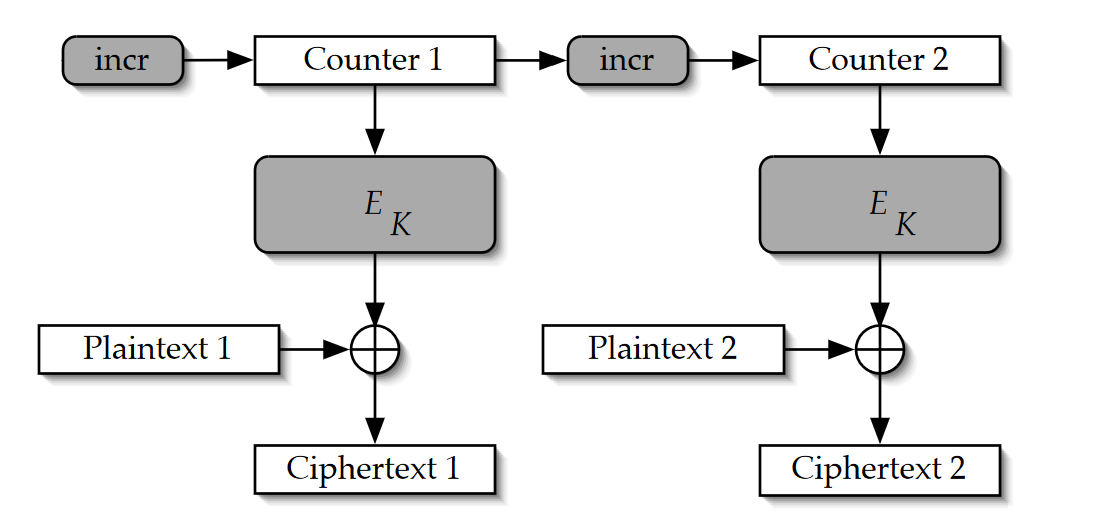
\includegraphics[scale=0.65]{resources/AES_counter.png}
    \caption{Counter part of the AES-GCM, src: The Galois/Counter Mode of Operation (GCM)~\cite{GCM_NIST}}
\end{figure}

\subsubsection{AES Counter}

The AES-GCM scheme consists of two main components. Firstly, there's the AES block encryption, resembling AES-CBC mode with certain adjustments. Secondly, there's the generation of the authentication tag, which authenticates the cryptogram and ensures its integrity. This module facilitates the computation of the first part, enabling the calculation of the cipher.


Here are the different functions of this module:
\begin{itemize}
    \item \texttt{incr\_iv(iv) -> iv}: increments the 32-bit counter part in the IV.
    \item \texttt{aes\_counter\_iv(ptr\_plain, ptrout\_cipher, length, key, iv)}: performs the AES-128 encryption on each 128-bit block of the input \texttt{ptr\_plain} using the counter mode with the IV \texttt{iv}, and sets the output using the pointer \texttt{ptrout\_cipher}. If the plain is not a multiple of 128 bits (last block is not a full block), then the last block is padded with zeroes.
    \item \texttt{aes\_counter(ptr\_plain, ptrout\_cipher, length, key)}: in this variation, the user does not specify an IV. It is instead randomly generated.
\end{itemize}

\subsubsection{GHASH}

GHASH is a cryptographic function used in the Galois/Counter Mode (GCM) encryption algorithm. It performs polynomial multiplication over a finite field with all authentication data and cipher blocks to generate an authentication tag for data integrity. This tag ensures that the data hasn't been tampered with during transmission. GHASH is an essential part of GCM, providing both encryption and authentication capabilities in a single operation.

Here are the different functions of this module:
\begin{itemize}
    \item \texttt{bit\_reflect(x) -> res}: inverts all the bits of the input \texttt{x} and returns the result \texttt{res}.
    \item \texttt{mult(a, b) -> res}: multiplies the inputs \texttt{a} and \texttt{b} in the Galois field $GF(2^{128})$ defined by the polynomial $x^{128} + x^7 + x^2 + x + 1$ and returns the result \texttt{res}.
    \item \texttt{ghash(a, b) -> res}: computes the GHASH operation on the inputs \texttt{a} and \texttt{b} and returns the result \texttt{res}.
    \item \texttt{ghash\_xor(ghash\_prev, data, h) -> res}: applies XOR to the inputs \texttt{ghash\_prev} and \texttt{data}, then computes the GHASH operation on the result and the input \texttt{h}, and returns the result \texttt{res}.
\end{itemize}

\subsubsection{AES-GCM}

This module serves as the core component of the project, aiming to integrate all the different elements of AES-GCM and thereby complete the encryption process.

Here are the different functions of this module:
\begin{itemize}
    \item \texttt{compute\_hash\_key(key) -> hash\_key}: computes the hash key, which is the enciphered zero 128-bit string using AES. The hash key is a recurring input of the GHASH function.
    \item \texttt{compute\_enciphered\_iv(key, iv) -> enc\_iv}: enciphers the IV (with counter 0) using AES. The enciphered IV is used to compute the authentication tag at the end.
    \item \texttt{compute\_length\_str(length\_auth\_data, length\_plain) -> length\_str}: computes the length string, which has a size of 1 block (128 bits). We will use the length string to compute the authentication tag. The 64 first bits are the length of the authentication data in bits. The 64 last bits are the length of the plain in bits. The inputs are in bytes.
    \item \texttt{ghash\_series(prev\_ghash, ptr\_data, length, hash\_key) -> ghash}: applies GHASH on each block of the data. It takes the previous GHASH value, the pointer to the data, the length of the data, and the hash key as input. It returns the new GHASH value.

    \item \texttt{aes\_gcm(ptr\_args, length\_auth\_data, length\_plain)}: the main function that performs the AES-GCM encryption and authentication. It takes the pointers to the arguments (key, iv, ptr\_auth\_data, ptr\_plain, ptrout\_auth\_tag, ptrout\_cipher), the length of the authentication data and the length of the plain as inputs. It writes the authentication tag and the cipher to the output pointers.
    \item \texttt{aes\_gcm\_inv(ptr\_args, length\_auth\_data, length\_cipher)}: the main function that performs the AES-GCM decryption and authentication. It takes the pointers to the arguments (key, iv, ptr\_auth\_data, ptr\_cipher, auth\_tag, ptrout\_plain), the length of the authentication data and the length of the cipher as inputs. It verifies the authentication tag and writes the plain to the output pointer. It returns 0 if the authentication tag has been successfully verified, and 1 otherwise.
\end{itemize}

\section{Further work}

So far, we have only implemented AES-GCM for 128-bit keys. It would be interesting to explore the extension of this implementation to include key sizes of 192 and 256 bits. This task could be complex because it involves direct manipulation of registers. Our first implementation required a delicate handling of the registers, and an implementation with larger keys might require the use of more registers, which would represent an additional challenge.

In addition, we validated our implementation of AES-GCM using test vectors from NIST~\cite{GCM_NIST} and a tool developed by GCHQ (Government Communications Headquarters)~\cite{GCHQ_git} for AES-GCM encryption, which ensures that our implementation is operational. However, we have not yet had the opportunity to conduct performance tests. A future job would therefore be to perform the first performance measurements of this implementation, optimize it, and then compare it to other existing implementations.

Finally, one of Jasmin’s main objectives is to develop "constant-time" codes to protect against possible attacks. We have verified that our implementation of AES-GCM complies with this requirement thanks to the "CheckCT" tool available within the Jasmin compiler. However, a new type of attack called Spectre~\cite{spectre} exploits vulnerabilities similar to cache attacks. Spectre takes advantage of speculative leaks in executing instructions to access sensitive data. To counter this threat, it is necessary to limit the branches, including while conditions and loops, as they can be exploited by Spectre. In our implementation of AES-GCM, we minimized the use of branches, which would facilitate the application of patches to ensure protection against this type of attack.

\section{Discussion}

Programming in Jasmin is challenging. Implementing an algorithm is not trivial because the programmer has more responsibilities than in higher-level languages. Jasmin's advantages (efficiency and verifiability) come at the cost of simplicity. Several noteworthy challenges can arise in the process of implementing a Jasmin program:

\begin{itemize}
    \item \textbf{Register Management:} Jasmin demands careful management of the number of registers, adding an additional layer of complexity to the programming task.
    
    \item \textbf{Operand Instructions:} The language introduces a distinctive feature where instructions with only two operands are permitted for registers of u8, u16, u32, and u64 types, further complicating the programming paradigm. However, instructions with three operands are permitted for u128 and u256.

    \item \textbf{Function Argument Constraints:} Function definitions in Jasmin are constrained to a maximum of six arguments, imposing limitations on the design and structure of functions.

    \item \textbf{Unclear Compiler Error Messages:} One of the obstacles faced is the lack of clarity in the error messages generated by the compiler. This can make debugging and troubleshooting a more challenging task.

    \item \textbf{Incomplete Documentation:} The available documentation for Jasmin is incomplete, making it imperative for programmers to navigate through the language's intricacies with limited guidance.
\end{itemize}

It is important to note that these observations are not intended as reproaches. Rather, they serve to illuminate the intricacies and challenges inherent in the process of working with Jasmin. Understanding these challenges is paramount, especially considering the relatively young and evolving nature of the Jasmin compiler, which was first released in 2021, just three years ago. Like any emerging technology, Jasmin is expected to undergo refinement and improvement in subsequent releases. As developers engage with Jasmin, they contribute to its evolution, shaping it into a more robust and efficient tool for programming tasks. Embracing these challenges fosters growth and innovation within the programming community, ultimately propelling the development of more sophisticated solutions in the ever-evolving landscape of technology.



\section{Conclusion}

In conclusion, the field of high-assurance cryptographic code remains crucial for safeguarding sensitive information in today's digital landscape. Specialized cryptographic programming languages like Jasmin offer a solid foundation for developing secure and efficient cryptographic implementations, with the Advanced Encryption Standard (AES) and its mode of operation, AES-GCM, serving as cornerstones for ensuring confidentiality and integrity.

However, the ever-present challenges posed by side-channel attacks underscore the importance of constant vigilance in the development of high-assurance cryptographic code. Mitigating vulnerabilities demands the adoption of constant-time algorithms, adherence to secure coding practices, and a proactive approach to addressing potential information leaks during execution.

Our exploration of cryptographic programming languages, particularly Jasmin, has shed light on both the strengths and challenges inherent in this domain. While Jasmin's unique combination of high-level and low-level features offers promise, its complexities, such as register management and operand instructions, present notable hurdles for developers.

Yet, these challenges are not insurmountable. With ongoing research and development, coupled with rigorous verification processes, the potential of Jasmin and similar languages to support the security of cryptographic systems remains substantial. By embracing these challenges and actively contributing to the refinement of cryptographic programming languages, we pave the way for enhanced security measures and more resilient digital infrastructures.

Looking ahead, there are clear avenues for further work in our project. Expanding the implementation of AES-GCM to support larger key sizes, conducting performance tests, and fortifying our code against emerging threats like Spectre are vital steps in advancing the state of high-assurance cryptographic code. Additionally, addressing the challenges inherent in programming with Jasmin requires a concerted effort to enhance documentation, improve compiler error messages, and provide better support for developers navigating its intricacies.

In essence, while the road ahead may be challenging, our endeavors in high-assurance cryptographic code stand at the forefront of securing digital communication and protecting sensitive information. Through collaboration, innovation, and a steadfast commitment to excellence, we can forge a future where cryptographic systems are not only robust but also resilient in the face of evolving threats.


% ---- Bibliography ----
%
% BibTeX users should specify bibliography style 'splncs04'.
% References will then be sorted and formatted in the correct style.
%
% \bibliographystyle{splncs04}
% \bibliography{mybibliography}
%
\newpage
\begin{thebibliography}{8}
\bibitem{hacl_star_paper}
Jean Karim Zinzindohouee, Karthikeyan Bhargavan, Jonathan Protzenko and Benjamin Beurdouche: HACL* A Verified Modern Cryptographic Library, Cryptology ePrint Archive, 2017 \url{https://ia.cr/2017/536}

\bibitem{qhasm}
Qhasm*, \url{https://cryptojedi.org/programming/index.shtml}. Last accessed 26 Jan 2024

\bibitem{cryptol}
Cryptol: The language of Cryptography \url{https://cryptol.net/files/ProgrammingCryptol.pdf}.

\bibitem{modified_AES}
Abikoye, Oluwakemi Christiana and Haruna, Ahmad Dokoro and Abubakar, Abdullahi and Akande, Noah Oluwatobi and Asani, Emmanuel Oluwatobi: Modified Advanced Encryption Standard Algorithm for Information Security. Symmetry 2019 \doi{10.3390/sym11121484}

\bibitem{random_generator}
Elaine Barker, John Kelsey: Recommendation for Random Number Generation Using Deterministic Random Bit Generators\doi{/10.6028/NIST.SP.800-90Ar1}

\bibitem{book_real_world_crypto}
David Wong.: Book: Real-World Cryptography. Manning,(2021)

\bibitem{jasmin_paper}
Almeida, Jos{\'e} Bacelar and Barbosa, Manuel and Barthe, Gilles and Blot, Arthur and Gr{\'e}goire, Benjamin and Laporte, Vincent and Oliveira, Tiago and Pacheco, Hugo and Schmidt, Benedikt and Strub, Pierre-Yves, Jasmin: High-Assurance and High-Speed Cryptography, CCS 2017 - Proceedings of the 2017 ACM SIGSAC Conference on Computer and Communications Security, Oct 2017, Dallas \url{https://hal.science/hal-01649140}.

\bibitem{vale_paper}
Bond, Barry and Hawblitzel, Chris and Kapritsos, Manos and Leino, K. Rustan M. and Lorch, Jacob R. and Parno, Bryan and Rane, Ashay and Setty, Srinath and Thompson, Laure, Vale: Verifying High-Performance Cryptographic Assembly Code, USENIX Association 2017 \url{https://dl.acm.org/doi/10.5555/3241189.3241261}.

\bibitem{GCM_NIST}
David A. McGrew, John Viega: The Galois/Counter Mode of Operation (GCM) \url{https://csrc.nist.rip/groups/ST/toolkit/BCM/documents/proposedmodes/gcm/gcm-spec.pdf}

\bibitem{paper_side_channel_attacks}
Antoine Geimer, Mathéo Vergnolle, Frédéric Recoules, Lesly-Ann Daniel, Sébastien Bardin, Clémentine Maurice: A Systematic Evaluation of Automated Tools for Side-Channel Vulnerabilities Detection in Cryptographic Libraries. arXiv e-prints 2023 \doi{10.48550/arXiv.2310.08153}

\bibitem{AES_NIST}
Morris Dworkin and Elaine Barker and James Nechvatal and James Foti and Lawrence Bassham and E. Roback and James Dray: Advanced Encryption Standard (AES). NIST FIPS 2001 updated 2023 \doi{10.6028/NIST.FIPS.197-upd1}

\bibitem{spectre}
M. D. Hill, J. Masters, P. Ranganathan, P. Turner and J. L. Hennessy: On the Spectre and Meltdown Processor Security Vulnerabilities \doi{10.1109/MM.2019.2897677}

\bibitem{GCHQ_git}
GCHQ: CyberChef \url{https://github.com/gchq/CyberChef}

\bibitem{cyber_in_nancy}
Cyber In Nancy 2022, \url{https://members.loria.fr/VLaporte/files/CyberIn2022.html}. Last accessed 29 February 2024

%%%%%%%%%% Formats examples
%\bibitem{ref_article1}
%Author, F.: Article title. Journal \textbf{2}(5), 99--110 (2016)

%\bibitem{ref_lncs1}
%Author, F., Author, S.: Title of a proceedings paper. In: Editor,
%F., Editor, S. (eds.) CONFERENCE 2016, LNCS, vol. 9999, pp. 1--13.
%Springer, Heidelberg (2016). \doi{10.10007/1234567890}

%\bibitem{ref_book1}
%Author, F., Author, S., Author, T.: Book title. 2nd edn. Publisher,
%Location (1999)

%\bibitem{ref_proc1}
%Author, A.-B.: Contribution title. In: 9th International Proceedings
%on Proceedings, pp. 1--2. Publisher, Location (2010)

%\bibitem{ref_url1}
%LNCS Homepage, \url{http://www.springer.com/lncs}. Last accessed 4
%Oct 2017
%%%%%%%%%%%

\end{thebibliography}


%\begin{figure}[ht] % ht = auto, H = fixed
%    \centering
%    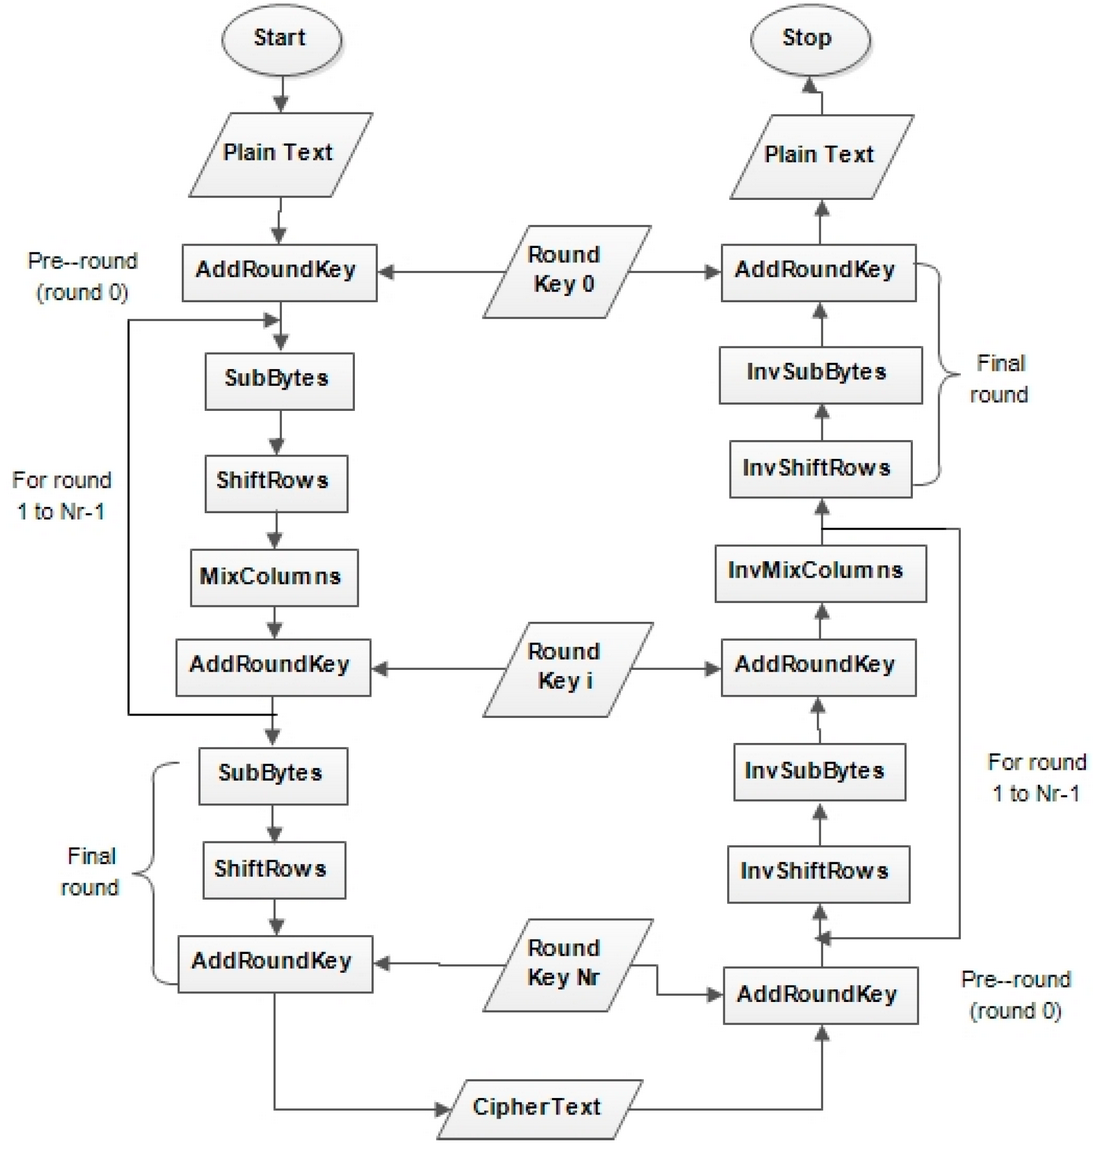
\includegraphics[scale=0.70]{resources/AES_schema.png}
%    \caption{Structure of the Advanced Encryption Standard (AES) %Algorithm. Src: \cite{modified_AES}}
%\end{figure}


\end{document}
